\capitulo{5}{Aspectos relevantes del desarrollo del proyecto}
En este apartado se pretende explicar las partes más significativas e importantes del desarrollo del proyecto, tanto su creación, diseño e interfaz gráfica, como las dificultades del mismo.

\section{Inicio del proyecto}
Tras hablar con José Ignacio y con Virginia de la posibilidad de realizar el TFG con ellos como tutores, comenzaron a pensar algún TFG que pudiesen ofrecerme. \\
En un inicio se valoró continuar con un trabajo anterior, desarrollado por un compañero en otro lenguaje, y ampliarlo de tal manera que se realizase un análisis de sentimientos y se implementase la nueva API de investigación de Twitter. Tras una reunión con los tutores, se decidió desarrollar desde cero una nueva aplicación, debido a que preferimos la opción de programarlo con un lenguaje aprendido durante los últimos años de carrera, para profundizar sobre él y facilitar su desarrollo. \\
\\\
Una vez iniciado el proyecto y habiendo tenido una primera reunión de toma de contacto, se presentó Silvia Díaz de la Fuente, investigadora predoctoral que se encuentra realizando una tesis sobre la gestión del patrimonio cultural en el Camino de Santiago Francés en Castilla y León. Con ella se va a realizar el proceso del desarrollo del proyecto ya que facilita la información más técnica del TFG.
\\\
\section{Primeros pasos}
Durante esta etapa se comienza investigando qué \textit{framework} utilizar. En un principio me decanté entre .NET y Django. La primera opción se descarta, ya que no es el mejor framework para el lenguaje Python, y la segunda opción resulta más atractiva para proyectos más grandes y robustos. Una opción parecida a Django pero más sencilla de utilizar es Flask, y dados los motivos explicados en el apartado anterior se decide decantarse por esta opción.
Además, se investigó sobre las herramientas que se iban a utilizar en un principio en el desarrollo de la aplicación y también sobre la API de Twitter, de la que se iba a extraer la información con la que trabajar durante el TFG.

\section{Formación}
Las herramientas y plataformas sobre las que se estudió su funcionamiento han sido:
\begin{itemize}
    \item \textbf{API de Twitter:} \\
    El proyecto de TFG XacoMeterII se enfoca en la implementación de la API de Twitter para la extracción de datos relevantes. Antes de iniciar la implementación, se llevó a cabo un análisis y evaluación de la funcionalidad de la API de Twitter y las distintas alternativas disponibles para su integración.\\
    Este análisis incluyó la identificación de los recursos y métodos de la API de Twitter que serían necesarios para el proyecto, así como la evaluación de las restricciones y limitaciones de la API. También se consideraron las diferentes alternativas de integración, bibliotecas y las técnicas de autenticación.\\ 
    Además, se realizó una evaluación de la documentación y los recursos de apoyo disponibles, incluída la comunidad de desarrolladores. Al final se decidió realizar la conexión a través de la librería \textit{'requests'}, ya que es una biblioteca más genérica y versátil que se puede utilizar para hacer peticiones HTTP a cualquier servicio web, no solo a la API de Twitter, y así entender bien el funcionamiento de conexión con las APIs.\\
    \item \textbf{Flask, .NET, Django:}\\
    Se eligió utilizar Flask como \textit{framework} para la creación de la aplicación debido a su facilidad de uso e instalación. Flask permite crear un servidor en Python de manera rápida y eficiente, y es una buena opción para proyectos de tamaño mediano y pequeño. Además, su diseño favorece el patrón de arquitectura MVC, lo que facilita la separación clara entre el modelo, la vista y el controlador.\\
    Aunque también se consideró la opción de utilizar Django o .NET, se decidió optar por Flask debido a su enfoque en proyectos más pequeños y simplificados. Django y .NET son marcos de trabajo más completos y orientados a proyectos de mayor escala. En este caso, Flask se adaptaba perfectamente a las necesidades y requerimientos de la aplicación.
    \item \textbf{Matplotlib, Plotly:}\\
    En un primer momento, se decidió utilizar la librería \textit{'Matplotlib'} para la generación de gráficos en el proyecto XacoMeterII, debido a la familiaridad con la misma, adquirida a través del uso previo en diversas asignaturas del grado.\\ 
    Sin embargo, con el avance del proyecto se consideró que sería más adecuado utilizar la librería \textit{'Plotly'} para la generación de gráficos interactivos.\\
    Para ello, se realizó una investigación en la página web de Plotly para adquirir conocimiento sobre su funcionamiento y características. Plotly es una librería de gráficos interactivos y visualización de datos que permite crear gráficos atractivos y fácilmente interactuables, y es ampliamente utilizada en aplicaciones web y móviles.\\
    Al usar Plotly, se pudo mejorar la representación visual de los resultados obtenidos a través de la extracción de datos de la API de Twitter.

\end{itemize}
\section{Metodología}
La metodología adoptada en este proyecto es SCRUM, aprendida en la asignatura de Gestión de Proyectos. Se basa en la aplicación de la metodología ágil para la gestión del proyecto, dividiendo el tiempo en periodos iterativos conocidos como \textit{"Sprints"}, en los cuales se establecen los objetivos y se realiza una estimación del coste temporal utilizando Story Points. 
\\La herramienta Zenhub ha sido utilizada para este proceso, ya que proporciona una plataforma de trabajo visual donde se puede interactuar con las tareas de manera sencilla y generar los gráficos.\\

En cuanto a las reuniones, se han realizado aproximadamente cada dos semanas. En ellas se llevaba a cabo una revisión del trabajo realizado, evaluando el progreso e identificando los objetivos cumplidos, la retrospectiva de dicho Sprint, exponiendo los problemas encontrados e identificando los aspectos a mejorar y la planificación del siguiente para establecer los objetivos a alcanzar y estimar el trabajo requerido para cada tarea.


\section{Desarrollo del proyecto}
\subsection{Implementación de la API de Twitter}
Una vez investigadas las herramientas que se iban a  poner en uso, se pudo comenzar a implementar la API de Twitter. En un inicio se realizó la conexión con la API a través de la herramienta \textit{Tweepy} y probando con un acceso \textit{'Essential'}, el cual solo permitía recoger los tweets más recientes.\\
Una vez implementado con el acceso más básico, se organizó una reunión con los tutores, y Virginia, al tener una página web en la que se la reconocía como docente de la Universidad de Burgos, pudo solicitar el acceso como investigadora a la API. Para ello contactó a través de la plataforma de \textit{Twitter developers} con Twitter y consiguió obtener las credenciales necesarias para realizar la conexión.\\
Se intentó durante un sprint conectar con la API a través de los nuevos datos de acceso, pero no hubo resultado.\\
Este paso causó varios problemas, ya que aplicando varios métodos de conexión no se obtuvo la respuesta esperada de la API de Twitter. Esto ralentizó mucho el proceso del desarrollo del proyecto, por lo que se decidió realizar otra reunión y tras revisar bien todos los pasos, se descubrió que no se había activado correctamente el nuevo acceso. \\
Al final se implementó la conexión con la API de Twitter mediante el uso de la biblioteca \textit{'requests'} en Python. Se definen varias funciones en el fichero \texttt{Code/FuncionPrincipal\_XacoMeterII.py} encargadas de autentificarse, acceder a los encabezados, realizar la solicitud a la API y conectarse a la API para obtener los datos deseados.\\
\begin{itemize}
    \item La función \textbf{auth} se encarga de devolver el \textit{token} de autenticación, el cual es un valor almacenado en una variable de entorno. La función 'accederEncabezados' recibe el token y devuelve los encabezados necesarios para la solicitud a la API, que incluyen la autorización.
    \item La función \textbf{solicitudURL} recibe como argumentos la palabra clave a buscar, la fecha de inicio y la fecha de fin, y devuelve la URL de \textit{endpoint} y los parámetros de búsqueda para la solicitud.
    \item La función \textbf{conexionEndpoint} es la encargada de realizar la solicitud a la API y devolver la respuesta en formato JSON. Recibe la URL del \textit{endpoint}, los encabezados y los parámetros de búsqueda.
    \item Finalmente, la función \textbf{funcionPrincipal} define las variables y hace las llamadas a las funciones anteriores para obtener la información deseada. Devuelve un diccionario con los tweets obtenidos de la API de Twitter para poder incluirlos en la base de datos PostgreSQL de manera sencilla a través de una query.
\end{itemize}

La API de Twitter con acceso de investigador académico tiene unas restricciones que han hecho que el proceso sea mucho más lento de lo esperado en un principio (Figura 5.1)\\
\begin{figure}[h!]
    \centering
    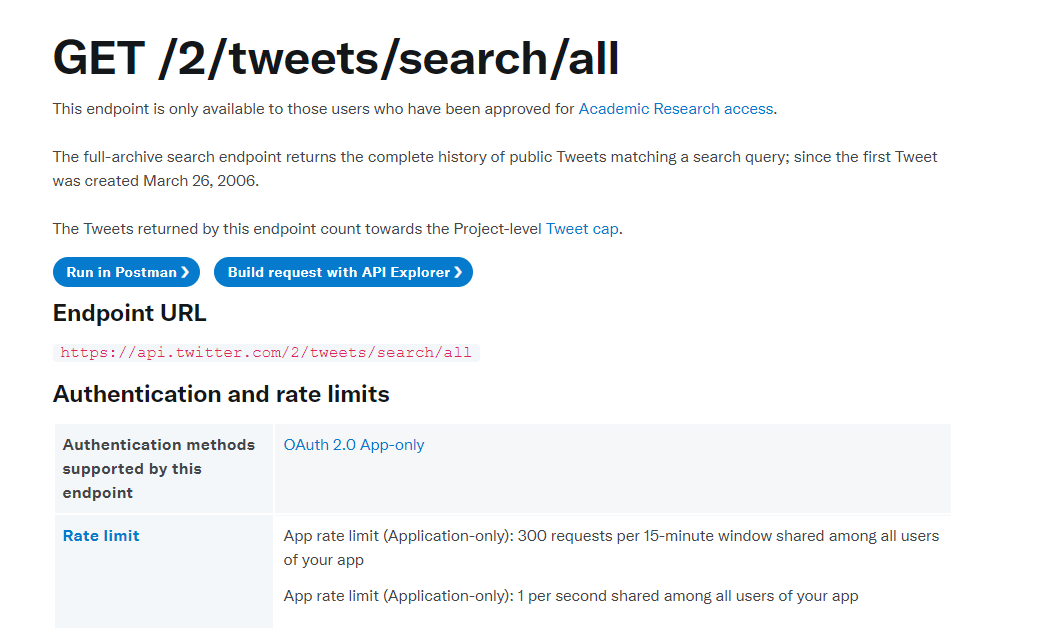
\includegraphics[scale=0.5]{img/SearchAll.png} \\
    \caption{Aspectos relevantes - API Twitter}
    \label{Aspectos relevantes - API Twitter}
\end{figure}
\begin{enumerate}
    \item Solo se pueden realizar 300 consultas cada 15 minutos.
    \item Cada petición debe durar mínimo 1 segundo.
    \item En cada petición se pueden obtener máximo 150 tweets.
\end{enumerate}
Así se ha tenido que configurar la parte del administrador, quien recopila los datos, de tal manera que introduzca unos parámetros para la búsqueda, para que en un futuro no se deba cambiar el código en el caso de que cambien las restricciones y con ellos, realizar paradas de tiempo (Figura 5.2).\\
\begin{figure}[h!]
    \centering
    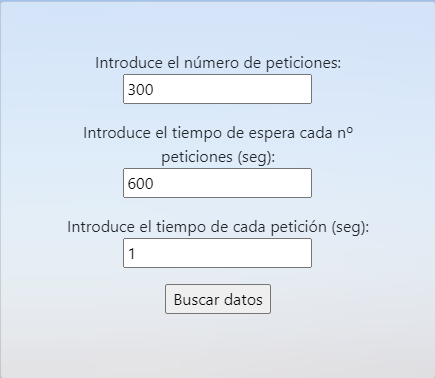
\includegraphics[scale=0.5]{img/parametrosBusqueda.png} \\
    \caption{Aspectos relevantes - Parámetros administrador}
    \label{Aspectos relevantes - Parametros administrador}
\end{figure}
Como en cada petición solo se pueden obtener 150 tweets y hay BICs que obtienen bastantes datos al día, se ha decidido realizar una petición al día por cada BIC, lo que quiere decir, que mínimo se van a realizar 130 peticiones para recopilar datos de un día completo de todos los BICs.\\
Actualmente solo se podrán realizar máximo 300 consultas cada 15 minutos y cada una de ellas debe durar mínimo 1 segundo. Además, se podrá calcular el tiempo de espera entre las consultas especificadas en el primer parámetro y las siguientes consultas. Twitter ha definido que se podrán realizar máximo 300 consultas cada 15 minutos, por lo que se recomienda esperar 10 minutos, es decir, 600 segundos:\\
    $$ 15\hspace{0.5em}minutos\times60\frac{\text{segundos}}{\text{minuto}}=900\hspace{0.5em}segundos $$
    $$ 300\hspace{0.5em}peticiones\times1\frac{\text{segundo}}{\text{petición}}=300\hspace{0.5em}segundos $$
    $$ 900\hspace{0.5em}segundos\hspace{0.5em}-\hspace{0.5em} 300\hspace{0.5em}segundos\hspace{0.5em}=\hspace{0.5em}600\hspace{0.5em}segundos$$
Twitter ha anunciado recientemente que se está realizando un cambio en su política de acceso a su plataforma a partir del 9 de Febrero. En lugar de ofrecer acceso gratuito a su API, Twitter implementará un nivel con una tarifa básica para su acceso (Figura 5.3).\\
\begin{figure}[h!]
    \centering
    
\includegraphics[scale=0.5]{img/TwitterDev.png} \\
    \caption{Aspectos relevantes - Comunicado Twitter}
    \label{Aspectos relevantes - Comunicado Twitter}
\end{figure}
\subsection{Creación y conexión de la base de datos}
Primeramente, para probar el funcionamiento de la API, se creaba un csv en el que se almacenaban los datos y así se podía comprobar si verdaderamente estaba realizando las operaciones correctamente.\\ Una vez comprobado, se procedió a crear una base de datos para almacenar la información. \\
Se quería utilizar una base de datos en la nube, pero tras buscar entre varias opciones, o no tenían gran capacidad de almacenamiento, o no eran en la nube. Debido a estas dificultades, se decidió utilizar una base de datos que pudiese ser desplegada en la nube, por lo que nos decantamos por PostgreSQL.
En un inicio, se comenzaron creando dos tablas en la base de datos local, y que, a partir del csv temporal se introdujesen los datos en PostgreSQL. Estas dos tablas eran la tabla en la que se almacenasen los nombres de los patrimonios con un id identificativo y la tabla en la que se guardase toda la información obtenida de la API de Twitter, con una clave foránea del id del nombre del BIC que se conectase con la tabla de nombres.

\subsection{Desarrollo de la parte visual del proyecto}
Una vez se tuvo la conexión con la API y la base de datos montada, se decidió crear una interfaz gráfica muy sencilla para ver algún resultado. Lo único que se desarrolló fue una nube de palabras donde se destacasen las palabras clave de los textos y un inicio con el nombre del proyecto. 
A lo largo del proyecto se fueron decidiendo aspectos que se querían incluir en la interfaz.
A partir de aquí, se fue ampliando de tal manera que:
\begin{enumerate}
    \item Primero, se decidió poner varios botones que permitiesen manejar la API, pidiéndola los tweets de todos los BICs marcando solo una fecha desde la que se requerían los datos. Esta acción, si la fecha era posterior a la primera fecha de la base de datos, borraba todos los registros entre las dos de la base de datos.
    \item La interfaz se fue mejorando y se incluyó que, además de crearlos desde una fecha, se pudiesen actualizar desde la última fecha registrada en la base de datos hasta la fecha actual.
    \item Al ver que la extracción de datos era bastante pesada, se decidió incluir un parámetro en la base de datos, booleano, en el que se marcase si el registro estaba eliminado o no, evitando de esta manera borrar registros de la base de datos y aumentando el rendimiento de extracción de datos de la API, ya que se no se tendrían que volver a solicitar dicha información.
    \item Estas acciones de actualizar o crear registros en la base de datos es un factor que pensamos que no todo el mundo debe controlar, por lo que decidimos que la mejor opción sería que solo un administrador con un usuario y una contraseña pudiese acceder, mientras que los usuarios generales solo pudiesen ver las estadísticas de los datos.
    \item Para que el inicio de sesión del usuario fuese seguro, primero se insertó en la base de datos un registro con el nombre de usuario y una contraseña encriptada.\\
    El usuario que desee realizar acciones de administrador deberá introducir un usuario y una contraseña, y si el nombre de usuario se encuentra en la base de datos, entonces se encripta la contraseña insertada y se compara con la de la base de datos. Solo en este caso se podrá acceder como administrador.
\end{enumerate}
\subsection{Creación de mapa didáctico}
Para las páginas accesibles para todos los usuarios, se comentó crear un mapa geográfico con los BICs ubicados en él. Primero se probó poniendo de fondo una imagen de un mapa y, sobre él, situar botones en los lugares más convenientes por pixeles. \\
Al ver que esa opción no estaba dando el resultado esperado, se pensó en implementar la API de Google, pero es una API de pago y se buscaron otras alternativas. \\
Al final, se encontró la herrmienta de \textit{'leaflet'}, que mediante coordenadas, permite insertar un mapa con un punto medio de visión y sobre él, se posicionan los marcadores por las coordenadas latitud y altitud situando todos los BICs a partir de datos almacenados en un csv (Figura 5.4).\\
También se pensó que, al haber 130 BICs, el mapa queda muy condensado, por lo que se podrían poner solo las localidades, y al hacer click sobre ellas, se redireccionase a una página con las imágenes de los patrimonios.\\
Silvia realizó una recopilación de imágenes relevantes para su investigación. Sin embargo, no disponía de las imágenes de todos los BICs y, debido a restricciones de derechos de autor si eran sacadas de internet se optó por no insertar imágenes.\\
Al final, se ubicaron todos los BICs en el mapa. 
Además, se implementó una funcionalidad de \textit{'popups'} en cada uno de los BICs, que incluía un enlace a la página donde se generan estadísticas específicas para cada bien. Se utilizó la función de hacer \textit{'hover'}, es decir, pasar el ratón, sobre el icono para mostrar el nombre del BIC sin necesidad de pulsar en cada uno de ellos.
\begin{figure}[h!]
    \centering
    \includegraphics[scale=0.3]{img/mapa.png} \\
    \caption{Aspectos relevantes - Mapa}
    \label{Aspectos relevantes - Mapa}
\end{figure}
\subsection{Creación de página de estadísticas}
Para la creación de la página de estadísticas, en un principio, se iba a insertar solo un gráfico temporal que mostrase el número de tweets publicados del BIC elegido en el mapa de todas las fechas almacenadas en la base de datos. \\
Estos gráficos se realizaron con la herramienta de \textit{'Matplotlib'} que facilita bastante la inserción de gráficos con el lenguaje Python.\\
Al tener bastantes datos en PostgreSQL, se decidió también crear otro tipo de gráficos. 
\begin{itemize}
    \item El gráfico temporal ya creado.
    \item Un gráfico circular que comparase los tweets del BIC seleccionado durante esa fecha respecto al total de tweets almacenados en la base de datos de todos los bienes históricos.
    \item Por último, resultaba interesante que al haber guardado las métricas públicas de los tweets, se pudiese realizar un gráfico de barras apiladas comparando los \textit{likes, retweets y replies} que se obtuvieron del BIC entre las fechas seleccionadas.
\end{itemize} 
Para poder realizar una búsqueda más específica, se añadió la opción de poder cambiar el rango de fechas para realizar las estadísticas, con dos calendarios en los que se puede seleccionar la fecha de inicio y de fin, siendo la primera fecha menor que la segunda.\\
En el caso de que no se inserte ninguna fecha, se utilizarán por defecto la primera fecha almacenada en la base de datos y la última.
\subsection{Despliegue con  Heroku}
Una vez se tuvo la aplicación montada en local, se comenzó el proceso de despliegue en Heroku. Para que la base de datos pueda ser accesible, también se añadió en Heroku un \textit{add-on} de Heroku-PostreSQL para desplegar la base de datos en la nube.\\
Para desplegar la base de datos se obtuvieron las credenciales de Heroku-PostgreSQL y se cambiaron en la aplicación por las que anteriormente habíamos insertado de la base de datos local. Además se configuró en PostgreSQL la nueva base de datos, transladando los datos anteriormente recuperados a través de un 'backup'.
\section{Mejoras}
Una vez completadas las funcionalidades básicas de la aplicación, se decidió mejorar la experiencia de usuario agregando una barra de navegación con una función de búsqueda para facilitar la interacción (Figura 5.5).\\

\begin{figure}[h!]
    \centering
    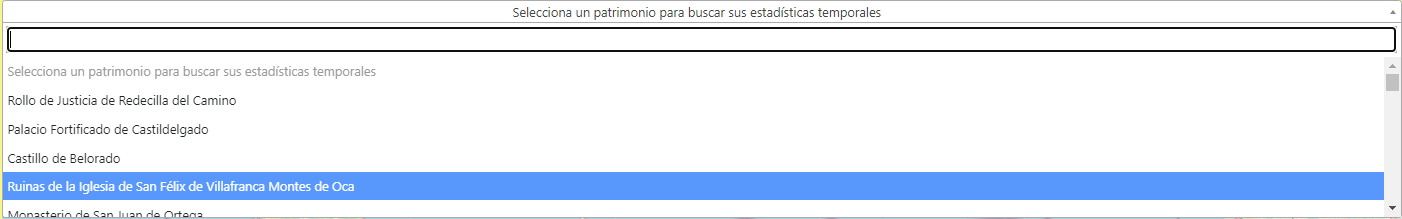
\includegraphics[scale=0.3]{img/busqueda.png} \\
    \caption{Aspectos relevantes - Barra navegadora}
    \label{Aspectos relevantes - Barra navegadora}
\end{figure}
Para garantizar la resolución de posibles errores en la aplicación, se implementaron mensajes de error para que los usuarios y el administrador puedan identificar y solucionar fácilmente los problemas (Figura 5.6).\\
\begin{figure}[h!]
    \centering
    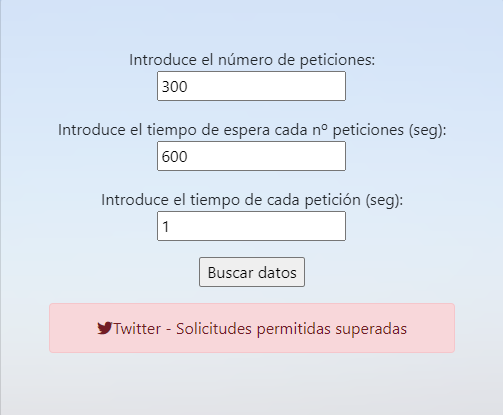
\includegraphics[scale=0.55]{img/errores.png} 
    \caption{Aspectos relevantes - Notificación de errores}
    \label{Aspectos relevantes - Notificación de errores}
\end{figure}
Para mejorar la presentación de los datos en la página de estadísticas, se implementó la librería \textit{'Plotly'} para generar gráficos interactivos, permitiendo al usuario realizar más acciones además de la visualización, como mover los gráficos.\\
Además, se incluyó una página de estadísticas temporales global con un gráfico de comparación de todos los BICs en un rango de fechas seleccionado (Figura 5.7).\\
\begin{figure}[h!]
    \centering
    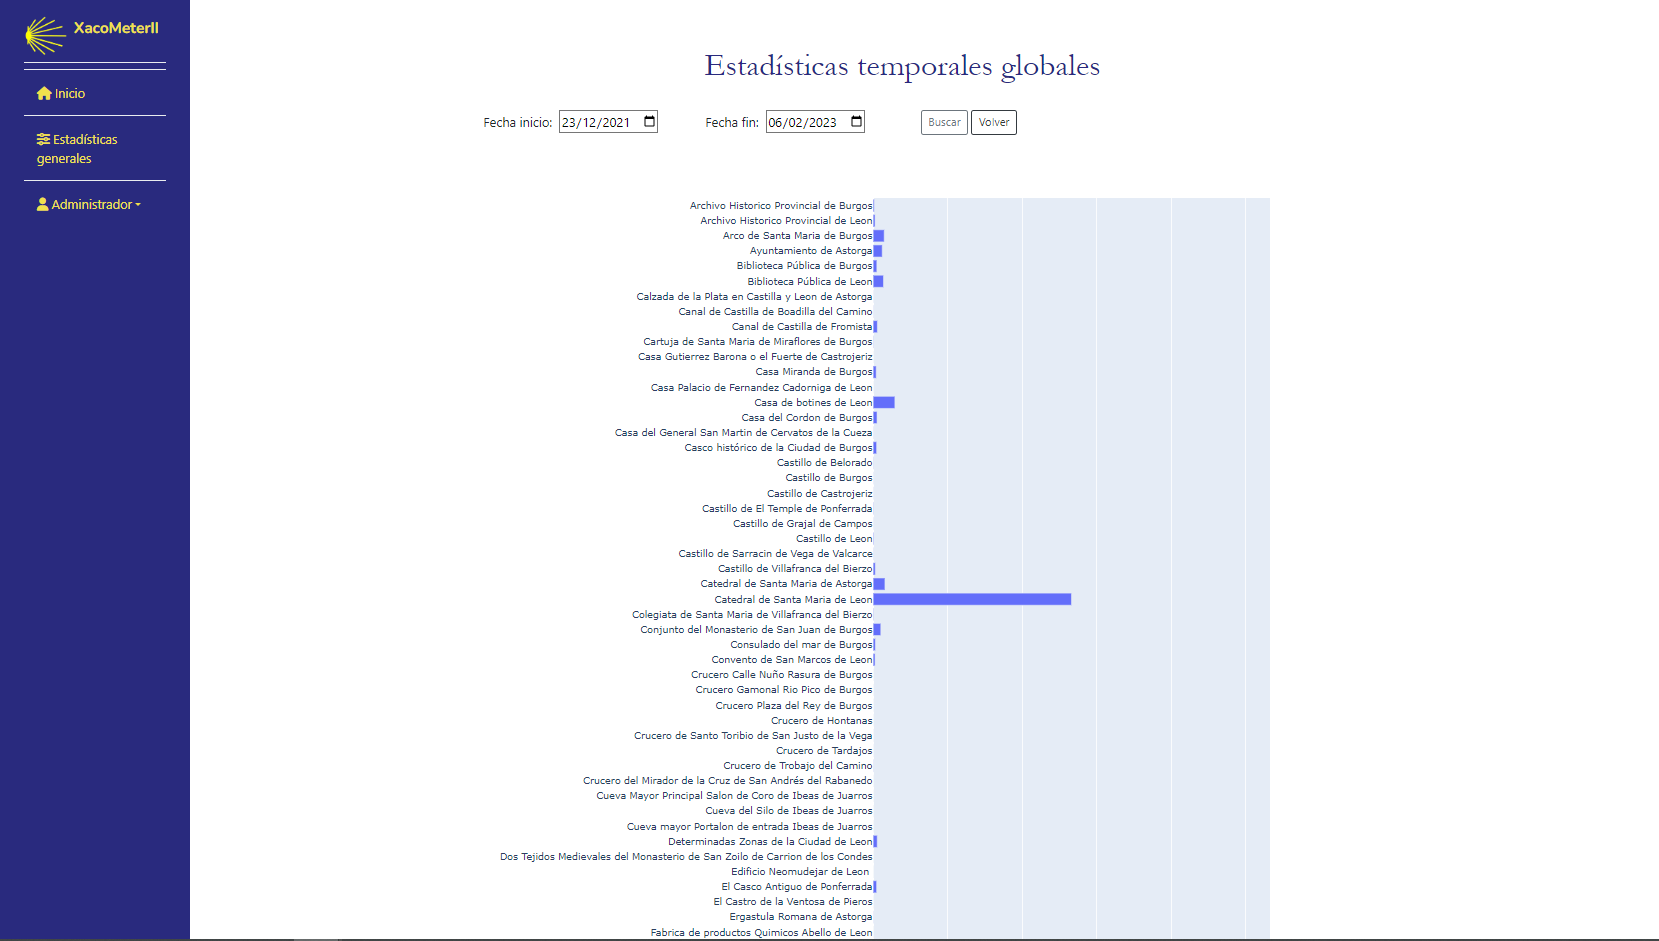
\includegraphics[scale=0.3]{img/EstadisticasGenerales.png}
    \caption{Aspectos relevantes - Estadísticas generales}
    \label{Aspectos relevantes - Estadísticas generales}
\end{figure}
\\
Por último, se agregó un análisis de sentimientos, que evaluará el sentimiento (positivo, neutral o negativo) en un número decimal entre 0 y 1, y se mostrará en un gráfico semicircular en la página de estadísticas del BIC. Se realizará una media de los sentimientos entre las fechas indicadas por el usuario (Figura 5.8).\\
\begin{figure}[h!]
    \centering
    \includegraphics[scale=0.3]{img/mejoras.png} \\
    \caption{Aspectos relevantes - Estadísticas mejoradas}
    \label{Aspectos relevantes - Estadísticas mejoradas}
\end{figure}